%\author{G.J. Lolos}
%\address{Dept. of Physics, University of Regina, Regina, SK, S4S 0A2 Canada}

\section{Aerogel \Cerenkov Counter}

\subsection{Overview}
Each High Resolution Spectrometer detector package includes a single silica 
aerogel
\Cerenkov counter of the compact reflection mirror design, which was 
dictated by the available space (36.3 cm along the incident particle direction). 
In addition, the high singles
rates expected in Hall A are better handled with segmented detectors
covering the focal plane, which requires short pulse
decay times.
  Even though the diffusion length in
silica aerogel can be quite short for low $\lambda$ light generated in the
$SiO_2$ radiator \cite{Lippert:1993kt}, enough directionality remains in the visible
$\lambda$ region, where the selected PMTs have good quantum efficiency, to make
light collection with mirrors an attractive and practical alternative. 

An effective segmentation of the aerogel \v{C}erenkov counter, matching the 
segmentation of the trigger scintillators, can be used to separate multiple
tracks through the focal plane and will allow an additional element of
selectivity and track sensitivity in the focal plane instrumentation.  This
means that specific sections of the focal plane can be physically disabled from
the trigger, if the experimental conditions require it.  It will also provide
the capability of identifying and separating pions and protons traversing the
focal plane trigger scintillators and the vertical drift chambers (VDCs) within
the resolving time of the system (double hits).  
For example, in the offline
analysis, the aerogel counter PMT with the highest number of photoelectrons can
be matched with the trigger counter and VDC information to identify the actual
path of a pion, thus separating it from a simultaneously detected proton, which
has no \Cerenkov signature.  Such a capability of double hit resolution is
not possible with diffusion \Cerenkov counter designs, because the photon
collection efficiency does not have a strong correlation with the incident
particle track within the aerogel material. 
 
The requirement for segmentation, in addition to supplementing the information
on the individual particle position along the focal plane, also couples well
with the desirability of increasing the active solid angle viewed by the PMTs
in the counter.  Although the photon detection probability is not as directly
proportional to the solid angle covered by PMTs as in the case of a diffusion
box, clearly, the larger the effective coverage, the higher the probability
will be that a photon will end up on a PMT.  Given the divergence of the beam
envelope incident on the aerogel, and the diffusion of the light in the low
$\lambda$ region by the aerogel material, an increase in the area covered by
PMTs results in an increase in the number of photons detected.  As a result, a
total of 26 PMTs are used in the counter, as shown in figure\ref{fig:aero_fig1}, with minimal
spacing between their $\mu$-metal shields (2.8 $mm$).  The total area covered
by the PMT photocathode windows comprises 72\% of the area of the counter
opposite the planar parabolic mirrors.  A cross sectional schematic of the
detector is shown in figure \ref{fig:aero_fig2}, clearly illustrating the planar parabolic design
of the mirror surfaces and their relative orientation with respect to the PMTs,
and the orientation of the counter relative to the central axis of the
spectrometers. 
   
The close spacing of the $\mu$-metal shields, which is also shown in the
photograph of figure \ref{fig:aero_fig3}, creates dielectric breakdown problems.  The $\mu$-metal
shields are at cathode potential (-2950 $V$) to avoid the capacitive discharge
from a grounded $\mu$-metal shield to the glass of the photocathode, which
would contribute to the noise level in the PMT, and adversely affect their
performance at high operating voltages. This necessitates extra precautions, in
order to avoid dielectric breakdown between adjacent shields, and between the
shields and the aluminum structure of the counter, which is at ground
potential. The solution was to wrap the outer surfaces of the $\mu$-metal
shields with a high dielectric value (12,000 $V/mm$), thin (0.254 $mm$) Teflon
film\footnote{DuPont Canada Inc., Box 2200, Streetsville, Mississauga, ON L5M 2H3, Canada.}.
  In addition, the PMT housings consist of fiberglass-epoxy
composites, with added inner and outer skins of 0.0254 $mm$ thick 
Tedlar\footnotemark[1],
with a further combined insulating value of 3,000 $V$.  Such a
combination of insulating materials eliminates any breakdown or small leakage
current induced noise and, at the same time, satisfies all safety requirements.

The final construction of the counter, described in this report, is built
around the two sides of the main (PMT) section, each consisting of two pieces
of aircraft quality aluminum alloy, with stiffening aluminum rods formed
integrally on the top and bottom.  The openings for the PMT housings were
machined on these structures using CNC milling machines to keep tolerances to
fine levels.  The double walled structure, on both sides of the enclosure,
further increases the rigidity of the exoskeleton by forming a second ``outer''
wall on each side, very similar in configuration to the inner one, and attached
to the latter with crossbolt braces, as shown in the photograph of
figure\ref{fig:aero_fig3}.
Each end plate is made out of the same aluminum alloy as the side walls, and
also incorporates stiffening lips folded integrally to each plate, one at the
top and one at the bottom.  Each end plate has been provided with inlet and
outlet gasline connections, which will be used to fill the counter enclosure
with dry $CO_2$ gas to protect the silica aerogel from water vapour absorption.
figures \ref{fig:aero_fig3} and \ref{fig:aero_fig4} show the bottom (tray) sections, 
and main plus upper (mirror)
sections, respectively.  The main (middle or PMT) section, in
figure \ref{fig:aero_fig4},
contains the PMTs and provides the strength and rigidity for the whole counter.
The one piece aluminum end plates are also shown in both photographs. 

All internal surfaces of the detector, except the planar parabolic mirrors,
themselves, are lined with aluminized 
mylar\footnote{National Metalizing, P.O. Box 5202, Princeton, NJ 08540, USA.} 
to increase the
overall reflectivity of the counter.  The mirrors are made in $45\times 20.5 
cm^2$ moulded surfaces, formed in one rigid structure. The rigidity is provided
by two layers of carbon fiber epoxy composite backing, with a combined
thickness of 0.28 $mm$, and a single sheet of mylar with thickness 0.127 $mm$. 
The special mylar material was obtained from exposed negative film used in the
cartographic industry, and is of high smoothness and uniformity.   One side was
aluminized at CERN, while the other side remains in its exposed negative
(black) state, further adding to the successive light penetration barriers into
the enclosure.   A representative reflectivity curve, as a function of
$\lambda$ for these mirrors, is shown in figure \ref{fig:aero_fig5}. 
 
The upper section of the counter containing the mirrors is mounted on its
own aluminum subframe, which is bolted to the main frame that houses the PMTs. 
The upper section, on its own, is shown in the photograph of
figure \ref{fig:aero_fig6}, while
its configuration when mounted on the main section is shown in
figure \ref{fig:aero_fig3}.  The
light and gas sealing action is provided by continuous twin parallel rubber
strips along the joint area, and by Tedlar film of 0.025 $mm$ thickness
covering the top of the outer planar parabolic area. 
\begin{figure}[p]
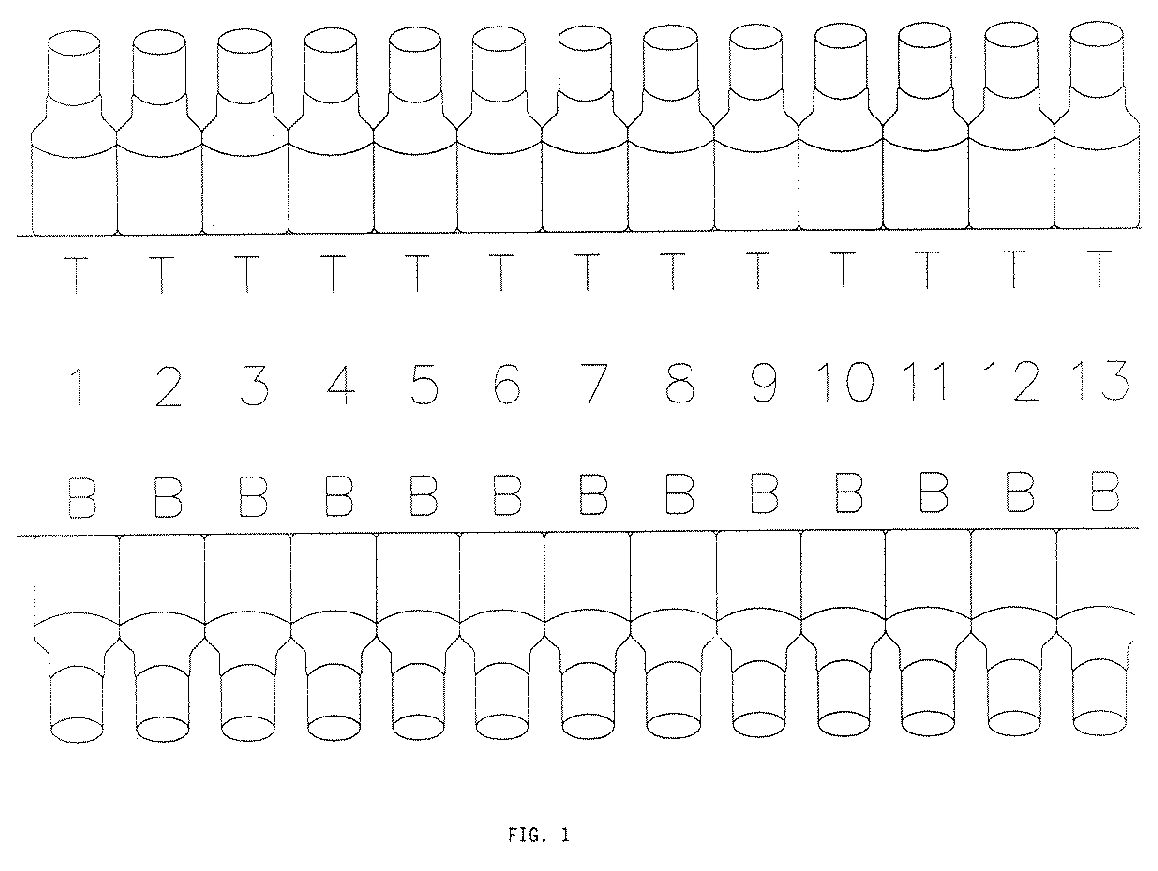
\includegraphics[angle=0,width=14cm]{aero_fig1}
\caption{
 Schematic diagram of the aerogel \v{C}erenkov counter as viewed by the
 incoming particles.  The numbers indicate the sections, 1 to 13, in the
 counter. Each section is viewed by two PMTs, one on the top (T) and one in the
 bottom (B). The labeling carries no significance other than identifying the
 PMTs during the testing phase, as described in the text.
 }
\label{fig:aero_fig1}
\end{figure}

\begin{figure}[tbh]
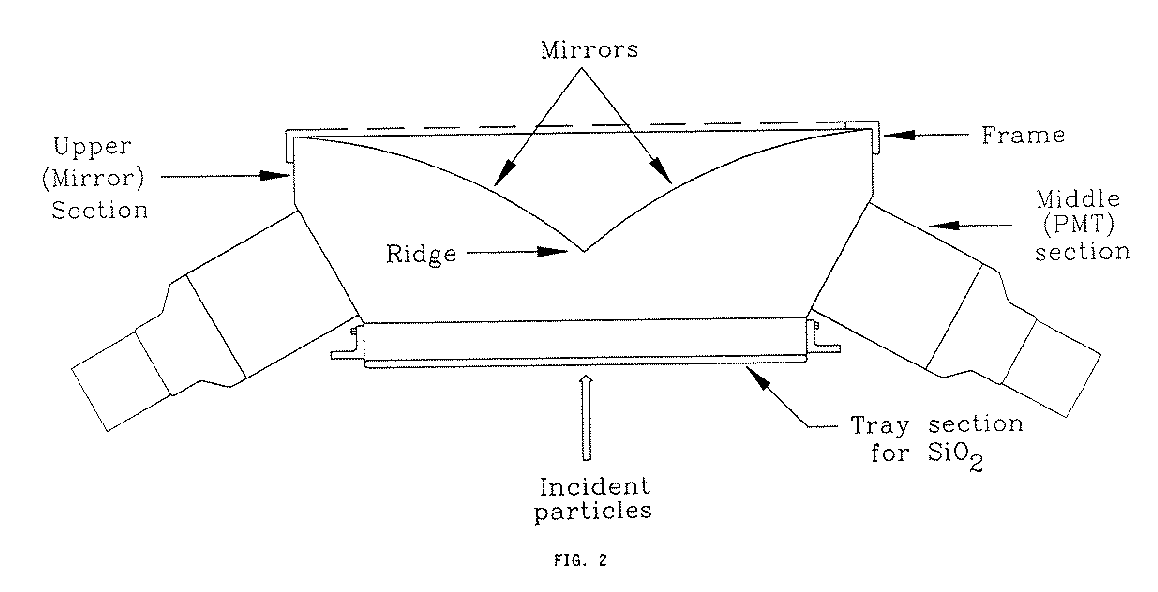
\includegraphics[angle=0,width=14cm]{aero_fig2}
\caption{
 Cross sectional drawing of the counter, along the particle direction, 
 showing the planar parabolic nature of the mirrors and the geometry of the 
 PMTs, as well as the final dimensions.  The joint of the two mirror surfaces in
 the middle of the counter defines the mirror ``ridge''.
 }
\label{fig:aero_fig2}
\end{figure}

The third major component of the counter consists of a removable tray where the
silica aerogel is placed. The tray occupies the bottom part of the counter and
has inside dimensions of $195\times 41 cm^2$ where the $SiO_2$ silica aerogel
is placed. It is formed by a frame with twin aluminum panels, which, in turn,
secure the removable frame strung with fishing line in a criss-cross pattern
to hold the aerogel panels in place.  This ``fishnet'' frame is secured by
screws and is easily removed without disturbing the aerogel panels or requiring
restringing.  The bottom of the tray is formed out of a single layer of carbon
fiber epoxy skin (0.127 $mm$ thick) and a layer of aluminized mylar of equal
thickness.  Externally, it is covered by a single layer of Tedlar film to
assure integrity from light penetration; further environmental isolation is
provided by two parallel strips of rubber gasket seals enclosing the
circumference of the tray and containing the feed-through spacers for the
retaining bolts.   The tray is equipped with SMA-type fiber optic feed through
connectors for the gain and timing monitor system, which utilizes fiber
optic cables.  Each fiber illuminates two adjacent PMTs, except the last PMT
on either side (13T and 13B in figure \ref{fig:aero_fig1}), which have their own dedicated fiber. 
The light is generated in a gas plasma discharge 
unit\footnote{Optitron Inc. 23206 S. Normandie Ave. \#8, Torrance, CA 90502, USA.} 
and
duplicates the spectrum expected from \v{C}erenkov radiation.  In addition, the
fibers terminate beneath the silica aerogel, thus, the light reaching the PMTs
will have the absorption characteristics of real \v{C}erenkov light produced 
in the aerogel radiator. 

Due to the nature of \Cerenkov detectors, where few photoelectrons (PEs) are
emitted by the photocathodes in the PMTs, any extraneous light entering the
enclosure is very troublesome.  As a result of the small number of PEs
expected, the PMTs operate either near to, or at, maximum high voltage, and,
thus, at maximum gain.  As such, they can suffer damage if a sudden light leak
develops.  In testing, we verified the extreme sensitivity to minute light
leaks, even across the whole length of the structure, because of the mirrored
surfaces inside the enclosure.  With 26 PMTs operating at maximum gain, and
viewing, effectively, a giant mirror, sealing the enclosure against single
photon penetration requires extra care during initial testing and operations.

The PMTs chosen for the counter were Burle model number 8854, 127 $mm$
photocathode 
diameter\footnote{Burle Industries Inc., 1000 New Holland Ave., Lancaster, PA 17601, USA.}.
  The PMT amplification electronics have
been described in Refs. \cite{Alexa:1995ne,Lolos:1997vz}.  The dynode chain incorporated a
600 $k\Omega$ resistance between the cathode and first dynode, instead of the
nominal 300 $k\Omega$.  This generates a $V_{dyn}=885 V$ across the cathode to
dynode gap, thus, increasing the photoelectron collection efficiency and peak
to valley (P/V) ratio.  This modification has been proven successful in
increasing the PE collection efficiency and the single PE resolution.  The
dynode amplification chain also incorporates a 11 $M\Omega$ resistor in series
with the $\mu$-metal shield to eliminate the possibility of electric shock
through careless handling; this high impedance also limits the current drawn,
in the unlikely event of a complete dielectric breakdown between the shields
and the aluminum parts of the detector. A schematic diagram of the electronic 
amplification chain is shown in figure \ref{fig:aero_fig7}. 

The operation of the aerogel detector is discussed in Ref.\cite{Brash:2002vn}.

\begin{figure}[p]

\includegraphics[angle=0,width=15cm]{blank}
\caption{
 Photograph showing the final arrangement of the double sidewall
 structure, and the close spacing of the housings for the PMTs.  The bottom
 section of the counter, with the tray and the aluminized mylar reflector
 lining, is also shown.  In this picture, the particles would be incident from
 the bottom toward the top of the counter.  The upper (mirror) section has been
 removed for clarity.
 }
\label{fig:aero_fig3}
\end{figure}

\begin{figure}[p]

\includegraphics[angle=0,width=15cm]{blank}
\caption{
 Photograph showing the middle (PMT) section with the double sidewall
 structures and the housings for the PMTs, with the top (mirror) section
 attached.  The tray has been removed, and the white tabs on the mirrors are
 pieces of tape holding a temporary protective film in place to prevent damage
 to the mirror surfaces during transportation.  In this figure, the particles
 would be incident from the top toward the bottom of the picture.
 }
\label{fig:aero_fig4}
\end{figure}

\begin{figure}[htp]
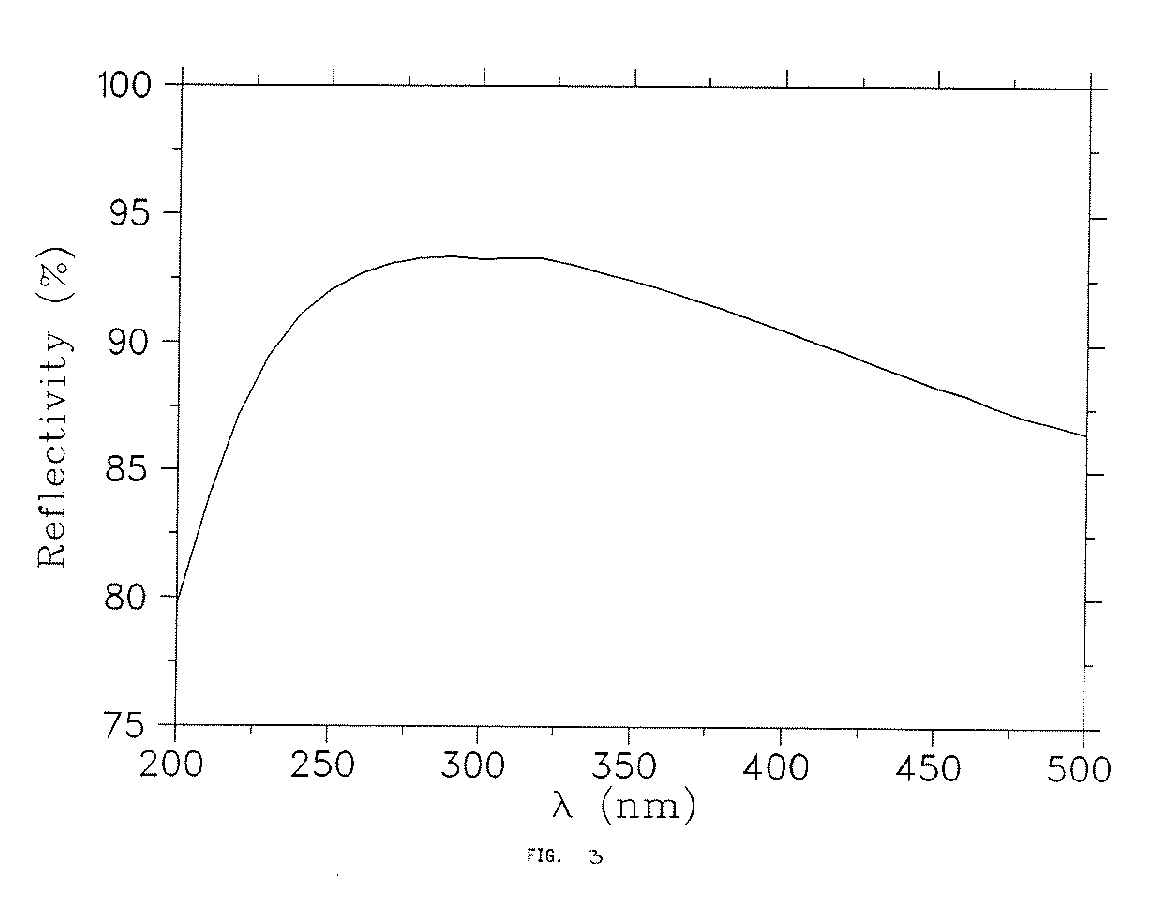
\includegraphics[angle=0,width=15cm]{aero_fig5}
\caption{
 Typical reflectivity curve of a mirror as a function of the 
 wavelength, $\lambda$, of the incident light.
 }
\label{fig:aero_fig5}
\end{figure}

\begin{figure}[p]

\includegraphics[angle=0,width=15cm]{blank}
\caption{
 A photograph showing the upper (mirror) section with the planar
 parabolic mirrors.  The mirror surface is protected by a vinyl film in this
 picture.  The mirror ``ridge'' separating the counter into two halves is
 clearly seen.  This section fits over the open top of the counter in Fig.\ref{fig:aero_fig3}.
 }
\label{fig:aero_fig6}
\end{figure}

\begin{figure}[p]

\includegraphics[angle=0,width=15cm]{blank}
\caption{
 Schematic diagram of the electronic amplification chain. The total 
 resistance of 600 $k\Omega$ between the cathode and the first dynode is shown 
 as three 200 $k\Omega$ resistors for sake of clarity. In the actual PC boards, 
 the arrangement is of six resistors of 100 $k\Omega$ each, in order to 
 keep the voltage across each resistor low and avoid surface discharge 
 between the closely packed resistors.
 }
\label{fig:aero_fig7}
\end{figure}

\subsection{Responsible Personnel} 
The following individuals are responsible for aerogel \Cerenkov problems. 
\begin{itemize}
\item[~]Serdarevi\'c, Maja - x5063
\item[~]Segal, Jack - x7242 
\item[~]Wojtsekhowski, Bogdan - x7191 
\end{itemize} 
 


\subsection{Safety Assessment}

The PMTs are under high voltage and care is required when handling any 
components of the counter. As stated earlier on in this report, the insulating 
material between the $\mu$-metal shield and the aluminum exoskeleton far 
exceeds the operating voltage. In addition, the 11 $M\Omega$ resistor between 
the $\mu$-metal shield and the HV source, restricts the current flow below the  
critical 1 $mA$ level. The combination of Tedlar film, plexiglas composites, 
and injection moulded bases, are all safe to handle but care should be 
exercised when handling the aluminum parts of the counter or touching the metal 
back plate of the base. It is strongly recommended to ground the aluminum 
exoskeleton of the counter, at several spots, to a common ground with the HV 
and signal cable ground. This will further enhance safety and eliminate 
potential ground loops in the unlikely event of a slow, and otherwise difficult 
to diagnose, dielectric breakdown from the $\mu$-metal shield to the aluminum 
structure or the aluminized mylar in the interior.  


\subsection{Operating Procedure}

\paragraph{Operating Voltage}
,

The operating voltage on the PMTs is -2,950 V. This is a near maximum rated 
voltage and it has been shown to combine high efficiency, good P/V ratio,   
and long PMT life. The overall gain of the PMT is not maximum, as is   
measured by BURLE, since the dynode chain of the 13 dynodes (2nd dynode to   
14th dynode) is kept at -2,600 V equivalent with the original 300 $k\Omega$   
resistor value between Cathode and 1st dynode. However, the gain is more   
than sufficient to separate the one PE from the pedestal of all ADCs we have   
used so far. It should not be necessary to increase the voltage above the   
recommended one. 


\subsection{Handling Considerations}


It is generally not advised to open up the counter if the persons involved are
not thoroughly familiar with the assembly and specific component function.
Routine operation does not require any hands on modifications to the detector,
as along as the following operating principles are followed: 

\paragraph{Installation and Removal of PMTs}

A replacement of a PMT or repairs of the electronic amplification chain can   
be accomplished by removal of that specific PMT-Base combination. Turn the   
HV off on all PMTs and remove the rubber hood covering the base and housing 
interface region. Now remove the three small screws attaching the base to   
the integral housing. Note that the base can only be secured to the housing   
in one specific orientation. 

Carefully slide out the base with the PMT and $\mu$-metal shield mounted as one
unit. Remove the elastomeric ring positioned between the PMT and the   
$\mu$-metal shield. Loosen the nut securing the $\mu$-metal shield to the   
base and carefully apply upward force on the shield while someone else is   
holding onto the base. This will remove the PMT and the $\mu$-metal shield   
from the socket and base, respectively. 

Replacement of the PMT requires experience because it has to be done with the
$\mu$-metal shield installed in, but not secured to, the base. The PMT pins
need to be aligned with the socket pins in a specific geometry, thus, the
insertion has to be done by feel and experience. Once the PMT is inserted in
the socket, the $\mu$-metal shield is secured the base with the nut. Make sure
the shield protrudes past the photocathode as much as the tapered design
allows. Carefully insert the elastomeric ring between the PMT rim and the
$\mu$-metal shield. This ring supports the PMT and prevents it from sliding 
out of the pins during movement; it also helps seal the interior of the counter
from the outside environment and reduces $CO_2$ leakage rate. 
Reverse the process for installation.

\paragraph{Installation and Removal of the $SiO_2$ Tray}

{\bf PLEASE NOTE}: The $SiO_2$ aerogel panels are extremely fragile and sensitive to 
water and chemical vapour. Do not handle with bare hands, use clean cotton, or 
other fabric type, gloves instead. Surgical gloves often are contaminated with 
lubricants and are not suitable for this purpose. 

The tray is secured to the main section by hex bolts. Removal of the bolts 
results in the straightforward removal of the tray. There is minimum clearance 
between the tray walls and the main section; as a result, the tray has to 
be removed and installed in a uniform translation with respect to the main 
body. The frame supporting the fish net (or tennis racket) can be removed from 
the tray proper by removal of the two small screws in the middle of the tray 
walls and a tool (hook) is provided for this operation. The $SiO_2$ aerogel 
panels can now be removed or replaced. Reverse the procedure for installation.
The securing bolts do not need to be tightened very much and, although spacers 
are inserted between the rubber strips to prevent damage, care and common sense 
 should be exercised. Light and gas sealing is provided by the 
rubber strips NOT by brute force.

{\bf WARNING}: After each removal of any components of the counter, check for light 
leaks before turning the HV on at operating values. Even a small light 
leak can destroy the PMTs if they are at -2,950 V! Check for light leaks with 
lights out, using a small portable light, and reduced voltage around -2,000 V.


\begin{table}
\caption{The number of photoelectrons detected as a function of PMT and 
incident beam location in the end plate proximity configuration.
$\Sigma^6 P.E.$ and $\Sigma^{26} P.E.$ denotes the measured total number of 
photoelectrons from six PMTS and the expected total from 26 PMTs, respectively. 
The incident electron beam location (hit position) is represented by
$[\times]$.} 
\begin{tabular}{lc|lc}
\multicolumn{4}{c}{PMT Location and Number of Photoelectrons}\\
\hline
1B $[\times]$ & 4.0 & 1T & 0.2 \\
2B            & 0.8 & 2T & 0.3 \\
3B            & 0.6 & 3T & 0.1 \\
\hline $\Sigma^6 P.E.$ & 6.0 & $\Sigma^{26} P.E.$ & 7.5\\
\end{tabular}
\label{tab:aero_tab1}
\end{table}

\begin{table}
\begin{tabular}{lc|lc}
\multicolumn{4}{c}{PMT Location and Number of Photoelectrons}\\
\hline
5B            & 0.5 & &  \\
6B            & 1.0 & 6T & 0.1 \\
7B $[\times]$ & 3.5 & 7T & 0.2 \\
8B            & 1.0 & 8T & 0.1 \\
9B            & 0.5 & & \\
\end{tabular}
\caption{As in table \ref{tab:aero_tab1}, but for the center hit location configuration.}
\label{tab:aero_tab2}
\end{table}




% ===========  CVS info
% $Header: /group/halla/analysis/cvs/tex/osp/src/hrs_det/aerogel.tex,v 1.2 2003/06/05 23:30:01 gen Exp $
% $Id: aerogel.tex,v 1.2 2003/06/05 23:30:01 gen Exp $
% $Author: gen $
% $Date: 2003/06/05 23:30:01 $
% $Name:  $
% $Locker:  $
% $Log: aerogel.tex,v $
% Revision 1.2  2003/06/05 23:30:01  gen
% Revision ID is printed in TeX
%
% Revision 1.1.1.1  2003/06/05 17:28:30  gen
% Imported from /home/gen/tex/OSP
%
%  Revision parameters to appear on the output
{\small
\begin{verbatim}CVS $Id: aerogel.tex,v 1.2 2003/06/05 23:30:01 gen Exp $\end{verbatim}
}
